% !TeX root = RJwrapper.tex
\title{\pkg{PDFEstimator}:  An R Package for Density Estimation and Analysis}
\author{by Jenny Farmer and Donald Jacobs}

\maketitle

\abstract{
This article presents \pkg{PDFEstimator}, an R package for nonparametric probability density estimation and analysis, as both a practical enhancement and alternative to kernel-based estimators. \pkg{PDFEstimator} creates fast, highly accurate, data-driven probability density estimates for continuous random data through an intuitive interface. Excellent results are obtained for a diverse set of data distributions ranging from 10 to $10^6$ samples when invoked with default parameter definitions in the absence of user directives. Additionally, the package contains methods for assessing the quality of any estimate, including robust plotting functions for detailed visualization and trouble-shooting. Usage of \pkg{PDFEstimator} is illustrated through a variety of examples, including comparisons to several kernel density methods. 
}

\section{Introduction} \label {intro}

The ability to estimate a probability distribution from a single data sample is critical across diverse fields of science and finance \citep{pdf1, pdf2, pdf3, pdf4}.  Estimating the parameters of the underlying density function becomes increasingly difficult when there is no prior information about the number of parameters, as the shape and complexity must also be inferred from that data. Although there are many nonparametric methods, kernel density estimation (KDE) is among the most popular.  

Variants of KDE differ based on how they implement the selections of the bandwidth and the kernel function, which are nontrivial decisions that can have a significant impact on the quality and performance of the estimate.  Most KDE implementations allow the user to manipulate some parameters manually, allowing for an experienced user to fine-tune the default behavior for improved results. Unfortunately, user directives introduce unavoidable subjectivity to the estimate.  More advanced implementations include intelligent and adaptive bandwidth selection optimized according to the characteristics of the data \citep{KDEtutorial, KDEdiffusion}. However, there is inevitably a trade-off between computational performance and accuracy \citep{KDEcomp}. There are many R packages available that can estimate density nonparametrically, typically based on KDE \citep{kdeR1, kdeR2, kdeR3, kdeR4, kdeR5, kernsmooth, densEstBayes, kde1d}. The core R function \code{density} implements a straightforward kernel density method.

Presented in this article is the package \CRANpkg{PDFEstimator} for nonparametric density estimation and analysis \citep{PDFe1}. The features of \pkg{PDFEstimator} can be separated into two categories. The first is a novel estimation method based on the principle of maximum entropy, available through the \code{estimatePDF} function. A primary advantage of \code{estimatePDF} is the automated interface, requiring nothing from the user other than a data sample. Range, multi-scale resolution, outliers, and boundaries are determined within the algorithm to achieve optimized data-driven estimates appropriate to the given sample. Although these defaults can be overridden by a sophisticated user, overrides generally do not improve the results. Additionally, multiple acceptable solutions can be returned, which is particularly useful in the case of low sample sizes where there is more statistical uncertainty.

The second category of features included in \pkg{PDFEstimator} is a unique set of assessment utilities for evaluating the accuracy of the solution and highlighting areas of uncertainty within a density estimate. Furthermore, a user-defined threshold can be specified to identify data points that fall outside of an expected confidence level. These diagnostics tools are visualized through a variety of customized plotting options, thus aiding in the evaluation of difficult distributions. Most importantly, all of these features can be applied towards any estimation function, such as \code{density}, as they are universal measurements independent of the method used, allowing for an integrated comparison between alternative models.

The remainder of this paper is organized as follows. ~\nameref{sec:usage} describes the functions available in this package, including their usage and underlying methods. ~\nameref{sec:examples} provides additional and advanced examples for identifying and troubleshooting problems with any density estimation method. ~\nameref{sec:comparison} compares \code{estimatePDF} with three popular kernel-based estimation packages using a diverse set of known distributions. Finally, ~\nameref{sec:stamps} demonstrates the use of \pkg{PDFEstimator} for a well-known real data set from a rare stamp collection.  

\section{Available functions and usage} \label{sec:usage}

An overview of the functions included in \pkg{PDFEstimator} is listed in Table~\ref{tab:functions}. A critical component of the tools in \pkg{PDFEstimator} is a \code{PDFe} object, which encapsulates all information necessary for plotting and assessing the quality of any density estimate. The member variables for the \code{PDFe} class definition are listed in Table~\ref{tab:pdfe}. The methods for calculating the necessary components of the \code{PDFe} and how they are employed in each of the functions in Table~\ref{tab:functions} are described in this section.

\begin{table}[t!]
\centering
\begin{tabular}{lp{10.4cm}}
\toprule
Function       & Description \\ \midrule
getTarget      & Returns upper and lower limits of SQR for a given target level \\
plotBeta       & Plots a shaded region outlining expected range of SQR values by position \\
estimatePDF    & Estimates a density from a data sample.  Returns a \code{PDFe}
                     estimation object. \\
convertToPDFe  & Converts any PDF to a \code{PDFe} estimation object for 
                     diagnostic purposes. \\
approximatePoints & Returns approximated PDF for an existing \code{PDFe} estimation object at a given set of data points. \\
plot           & Main plotting function for \code{PDFe} estimation objects. \\
lines          & Plots the density for a \code{PDFe} estimation object as a connecting                           line segment to an existing plot. \\ 
summary        & Prints a summary of the \code{PDFe} object. \\ 
print          & Prints the probability density and cumulative density for
                     each estimation point in the \code{PDFe} object.  \\ \bottomrule
\end{tabular}
\caption{\label{tab:functions} Overview of functions in the \pkg{PDFEstimator} package.}
\end{table}

\subsection{The PDFe class} \label{subsec:pdfe}

The first four member variables listed in Table~\ref{tab:pdfe} are commonly understood values for an estimated density, beginning with the random data sample that is the basis for the estimate. The probability density function (PDF) is estimated for the range of points defined in \code{x}. Similarly, the cumulative distribution function (CDF) can be calculated representing the cumulative probability of the PDF for each \code{x}. \pkg{PDFEstimator} defines additional descriptions for an estimate that measure the quality of its fit to the sample data. Central to the quality of these estimates is a scoring mechanism to rate the overall fit of an estimate to the sample. A single average score is calculated, as well as individual confidence levels for each data point within the sample. These scores are based on order statistics \citep{order}.

If the CDF, defined on the range (0 1), is an accurate representation of the data, then $CDF(x)$ will represent uniform random data. The general problem then becomes assessing if $r_k=CDF(x_k)$ represents uniform data for a given sample. Although there are many methods to test for uniform data \citep{PDFe2}, \pkg{PDFEstimator} employs an average quadratic z-score, defined as 
\begin{equation} \label{eq:zscore}
z^2=\frac{-1}{N} \sum_{k=1}^{N}\frac{\left(r_k-\mu_k\right)^2}{\sigma_k^2},
\end{equation}
where $k$ is the sort ordered position in a sample size $N$, and $\mu_k$ and $\sigma_k$ are the mean and standard deviation from single order statistics known to be $\mu_k=-\frac{k}{N+1}$ and $\sigma_k=\frac{\mu_k\left(\mu_k-1\right)}{\sqrt{N+2}}$. Perfectly uniform data would yield a score of exactly zero.

To study typical z-scores for uniform random data, extensive numerical experiments were generated with a random number generator on the range (0, 1) for many different sample sizes. The typical distribution of scores according to Equation~\ref{eq:zscore} is represented in the left plot for Figure~\ref{fig:scores}. The peak density of the PDF corresponds to the most likely z-score and occurs at a value of approximately -0.5, with a sharp drop-off in the density as scores approach zero. The \code{threshold} value of the \code{PDFe} object reports the empirical cumulative probability for the z-score, as a percentage, shown on the right-hand plot of Figure~\ref{fig:scores}. The cumulative probability for the peak z-score is calculated to be a little over 0.7, thus a threshold value near or greater than 70\% can be considered a highly probable fit. A threshold of less than 5\%, by contrast, is low probability and therefore likely an underfit for the data. In this event, the \code{PDFe} member variable  \code{failedSolution} is set to \code{TRUE}.  A score with a threshold of 95\%, however, is similarly unlikely and can be interpreted as overfitting the data. The software does not rigidly enforce a particular score upon an accepted solution, but rather uses the numerically calculated density shown in Figure~\ref{fig:scores} as a guide to iteratively move towards increasingly probable solutions. 

The threshold provides an average score for the estimate, but to assess the estimate per position and identify the locations of potential errors, a scaled quantile residual (SQR) is defined as
\begin{equation} \label{eq:sqr}
SQR_k=\sqrt{N+2} \left(r_k-\mu_k\right).
\end{equation}
The scaling factor of $\sqrt{N+2}$ creates a sample-size-invariant metric for each position $k$. The \code{sqr} member variable of the \code{PDFe} class contains a vector of SQR values according to Equation~\ref{eq:sqr} and their ability to diagnose problems in a density estimate will be demonstrated with the \code{plot} function. Note that the \code{PDFe} object will also report the size of \code{sqr}, which will be the number of samples less the number of any outliers detected.

\subsection{getTarget and plotBeta} \label{beta}

It has been shown that, when plotted against position, $SQR_k$ for uniform random data falls approximately within an oval shaped region \citep{PDFe2}. The reason for this can be understood by examining the beta distributions that govern order statistics for sort ordered random uniform data \citep{order}. The probability of $u$ for position $k$ in uniform random data with $N$ samples is as follows.
\begin{equation} \label{eq:beta}
p_k(u)=\frac{N!}{\left(k-1\right)!\left(N-k\right)!}u^{k-1}\left(1-u\right)^{N-k}
\end{equation}
By integrating Equation~\ref{eq:beta} for each position $k$, confidence levels for SQR values of sample size $N$ are calculated in the \code{getTarget} function. Figure~\ref{fig:sqr} demonstrates confidence levels for three different target percentages, plotted as contour lines. The background shading in grey represents typical ranges of SQR values, with darker shading corresponding to higher probability areas. This shading is independent of sample size, and is calculated according to Equations~\ref{eq:sqr} and ~\ref{eq:beta} in the \code{plotBeta} function.


\begin{table}[t!]
\centering
\begin{tabular}{lp{10.4cm}}
\toprule
Member Variable  & Description \\ \midrule
sample    & Sample data used to estimate the density. \\
x         & Points where the density is estimated. \\
pdf       & Estimated density values for \code{x}. \\
cdf       & Cumulative density values for \code{x}. \\
threshold & Threshold score, expressed as a percentage, measuring the uniformity of the  CDF of sample data.  \\
failedSolution & If true, indicates that the estimate returned does not meet at least a 5\% threshold. \\
sqr       & Scaled quantile residual values for sample data points. \\ 
sqrSize   & Size of sqr. \\ 
\bottomrule
\end{tabular}
\caption{\label{tab:pdfe} Member variables of the \code{PDFe} class.}
\end{table}

\begin{figure}[!htb]
\centering
\begin{tabular}{p{0.4\textwidth} p{0.4\textwidth}}
  \vspace{0pt} 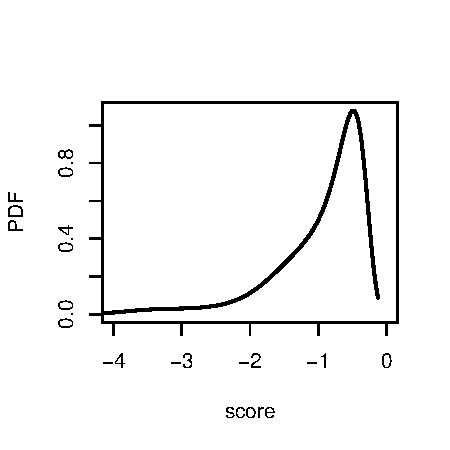
\includegraphics[width=2.0in, height=2.5in]{Figure1a.pdf} &
  \vspace{0pt} 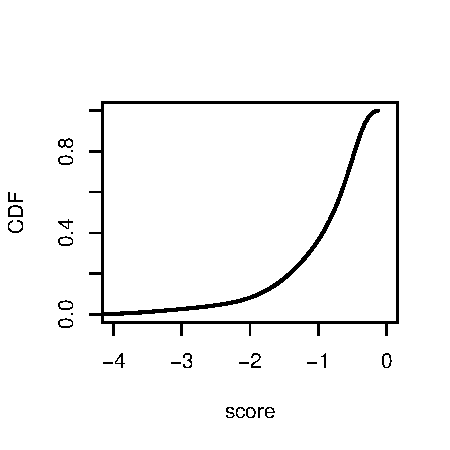
\includegraphics[width=2.0in, height=2.5in]{Figure1b.pdf} 
\end{tabular}
\caption{\label{fig:scores} These plots demonstrate the distribution of scores as defined by Equation~\ref{eq:zscore} and are used to assess the probability of a trial solution. The density was estimated empirically by generating 1000 trials of 10,000 uniform random data samples. The probability density function is shown on the left and the cumulative density function is on the right. }
\end{figure}

\begin{figure}[!htb]
\centering
\begin{tabular}{p{0.4\textwidth} p{0.4\textwidth}}
  \vspace{0pt} 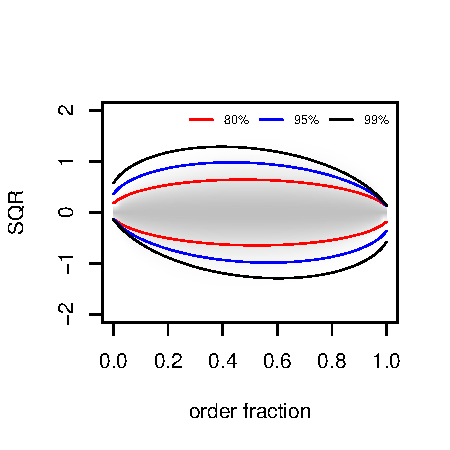
\includegraphics[width=2.0in, height=2.5in]{Figure2a.pdf} &
  \vspace{0pt} 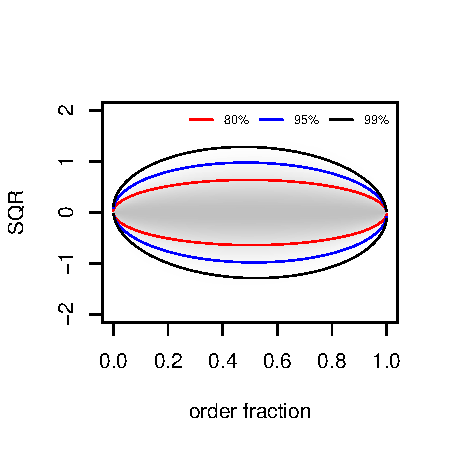
\includegraphics[width=2.0in, height=2.5in]{Figure2b.pdf} 
\end{tabular}
\caption{\label{fig:sqr} Confidence levels by position for a scaled quantile residual plot based on beta distribution probabilities according to single order 
statistics for a sample size of 50 (left) and 1000 (right). The colored contour lines define regions within an oval shape that give target levels for observing data points deviating away from perfect uniform spacing as expected for true uniform random data. Note that the skewness in the contour lines are noticeable for small sample sizes compared to large sample sizes.}
\end{figure}
\subsection{estimatePDF} \label{estimatePDF}

\code{estimatePDF} provides an R interface for nonparametric density estimation based on a novel method providing an alternative to traditional KDE implementations. Details of this approach, based on the principle of maximum entropy \citep{mem1}, were published previously and have been shown to produce more accurate estimates than KDE in most cases \citep{PDFe1, PDFe2, kdeR6, matlab}. For optimal performance and flexibility with other applications, this functionality is performed within a set of C++ classes and is not the focus of this paper, but a brief summary is provided for insight into the \code{estimatePDF} interface.

In a traditional maximum entropy method, moments for a set of characteristic  functions are introduced, and the coefficients to these functions are optimized to match the predicted moments with the empirical moments. As a particular choice of moments that exist for any probability density, and to form a systematic truncated expansion over a complete set of orthogonal functions, the analytical form for the density function from a data sample is expressed as 
\begin{equation} \label{eq:entropy}
p(\nu)=\sum_{j=1}^{D}\exp\left(\lambda_jg_j(\nu)\right),
\end{equation}
where $g_j(\nu)$ are bounded level functions and $\lambda_j$ are Lagrange coefficients controlling the shape of the density function \citep{mem2}. For a fixed number of coefficients, $D$, this method is parametric in form. Although solving for the coefficients analytically is increasingly impractical for high dimensionality, a random search method is employed that provides very
efficient numerical optimization. An expansion of orthogonal functions is constructed in the form of Equation~\ref{eq:entropy}, without specifying D in advance, where higher mode orthogonal functions are successively added as needed. The algorithm iteratively explores possible density functions by perturbing the Lagrange coefficients that are currently present, while D is slowly increased, testing each possibility according to the scoring function in Equation~\ref{eq:zscore} to converge towards an accurate estimate.

The arguments for \code{estimatePDF} are listed in Table~\ref{tab:arguments1}. If no other parameters are specified, the range of the returned estimate is calculated automatically.  By default, left and right boundaries are presumed theoretically infinite and allowed to extend beyond the range of the data sample. The finite numerical bounds are calculated according to the density near the tails, with longer tails receiving more padding than shorter tails.  Similarly, extreme outliers are detected and removed from the sample as appropriate according to the \code{outlierCutoff} argument.  Alternatively, the \code{lowerBound},  \code{upperBound}, and \code{outlierCutoff} parameters can be independently specified to provide the user complete control over the range of the estimate. Setting \code{outlierCutoff} to zero turns off outlier detection and includes all the data.


\begin{table}[t!]
\centering
\begin{tabular}{lp{10.4cm}}
\toprule
Arguments     & Description \\ \midrule
sample        & A vector containing the data sample to estimate.\\
pdfLength     & Specifies the desired length of the estimate returned. By default, this length is calculated based on the length of the sample. \\
estimationPoints & An optional vector containing specific points to estimate.\\
lowerBound    & Sets the finite lower bound for the sample, if it exists.\\
upperBound    & Sets the finite upper bound for the sample, if it exists.\\
lagrangeMin   & Specifies the minimum allowed dimension, $D$, in Equation~\ref{eq:entropy}. \\
lagrangeMax   & Specifies the maximum allowed dimension, $D$, in Equation~\ref{eq:entropy}. \\
debug         & If TRUE, detailed progress will be printed to the console.\\
outlierCutoff & If greater than 0, specifies the range of included sample data, according to the formula [(Q1 - outlierCutoff x IQR),  (Q3 + outlierCutoff x IQR)], where Q1, Q3, and IQR represent the first quartile, third quartile, and inter-quartile range, respectively. \\ 
target        & Sets a target percentage threshold between 0 and 100.
The default is 70, the minimum accepted is 5.\\
smooth        & If TRUE (default), preference is given towards smooth density estimates. \\ \bottomrule
\end{tabular}
\caption{\label{tab:arguments1} Overview of arguments in the \code{estimatePDF} function.}
\end{table}

The number of expansions in Equation~\ref{eq:entropy} begins at \code{lagrangeMin} and is capped at \code{lagrangeMax}, with default values of 1 and 200, respectively. The maximum of 200 provides a generous realistic upper limit to the complexity of the estimate and the computational time required but can be altered to either increase accuracy or decrease compute time. Another reason to override these limits is to create a semi-parametric estimate by narrowing the range between minimum and maximum.  A strictly parametric approach can be achieved by setting the two limits to the same value. For example, setting both \code{langrangeMin} and \code{lagrangeMax} to 1 forces a uniform fit. Similarly, setting them both to either 2 or 3 respectively yields exponential and Gaussian distributions.

The \code{target} argument refers to the cumulative probability of the z-score, as previously discussed. Note that \code{target} is a user-defined argument, whereas \code{threshold} in the \code{PDFe} class is the actual threshold achieved. These values may be different for several reasons.  For example, the search for the target threshold may abort prematurely if the \code{lagrangeMax} has been exceeded or if progress has been stalled.  Additionally, a small penalty is added to the score if the estimate becomes exceptionally noisy in areas of low density where sharp features are not justified. Therefore, a smoother curve may be favored over a higher score. The smoothing penalty is constructed according to a Taylor expansion error estimate as
described previously \citep{mem2}. The original model calculated a second order expansion, but a first order approximation was found to be sufficient and implemented in this version. This behavior can be circumvented when intentionally searching for small peaks by setting the \code{smooth} argument to FALSE.

\subsection{convertToPDFe and approximatePoints} \label{convert}

The \code{estimatePDF} function performs the density estimation based on the input parameters in Table~\ref{tab:arguments1} and returns a \code{PDFe} object for plotting and additional analysis. Alternatively, the \code{convertToPDFe} function will create a \code{PDFe} object for an estimate calculated using any other method for a given data sample. \code{convertToPDFe} requires a data sample and the \code{(x, y)} values for the estimate, and calculates the score, threshold, and SQR values for each point in the sample.

The \code{approximatePoints} function operates on a \code{PDFe} object to approximate the PDF for additional data points after the estimate has already been calculated using either \code{estimatePDF} or \code{convertToPDFe}. This functionality is similar to specifying \code{estimationPoints} in the \code{estimatePDF} function, but is provided for the convenience of approximating different points without having to recalculate the estimate. The following example will create a \code{PDFe} object for a KDE estimate of a random sample from a standard normal distribution, and then return additional density approximations at points -3, 0, and 1.

\begin{example}
    sample = rnorm(1000)
    kde = density(sample)
    pdfe = convertToPDFe(sample, kde$x, kde$y)
    approximatePoints(pdfe, c(-3, 0, 1))
\end{example}

\subsection{plot} \label{plotfunction}

The \code{PDFEstimator::plot.PDFe} function extends the generic \code{plot} function in R supporting all existing graphical parameters, with additional options summarized in Table~\ref{tab:arguments2}. The first argument listed in the table is the \code{PDFe} object returned by \code{estimatePDF} or \code{convertToPDFe} and is required for all plots. The \code{plotPDF} and \code{plotSQR} arguments can be independently set to TRUE or FALSE and collectively control the plot type. The \code{plotShading} and \code{showOutlierPercent} values invoke the \code{plotBeta} and \code{getTarget} functions from Table~\ref{tab:functions} and provide optional diagnostics to highlight specified uncertainties within the estimate through the use of the SQR plot. The remaining arguments listed in Table~\ref{tab:arguments2} control minor graphical features for  customized aesthetics.  The following examples will demonstrate the variety of plots that can be created with combinations of these options.


\begin{table}[htb!]
\centering
\begin{tabular}{lp{10.4cm}}
\toprule
Arguments     & Description \\ \midrule
x             & A \code{PDFe} estimation object. Returned from \code{estimatePDF}.\\
plotPDF       & Plots the probability density for x if TRUE. \\
plotSQR       & Plots the scaled quantile residual (SQR) for x if TRUE.  If plotPDF is also TRUE, the SQR will be scaled to the range of the density. \\
plotShading   & Plots gray background shading indicating approximate confidence levels for the SQR, where darker shades indicate higher confidence. Setting this to TRUE only has meaning when plotSQR = TRUE.\\
shadeResolution  & Specifies the number of data points plotted in the background shading when plotShading = TRUE. Increasing this resolution will create sharper and more accurate approximations for the confidence levels, but will take more time to plot. \\
showOutlierPercent  &  Specifies the threshold to define outliers for SQR.  Must be a number between 1 and 100.\\ 
outlierColor     & Specifies the color for outliers when showOutlierPercent is defined.\\
sqrPlotThreshold & Magnitude of y-axis for SQR plot. \\
sqrColor         & Specifies the SQR color for non-outliers\\
type             & Specifies the line type of the density curve if plotPDF = TRUE.  If plotPDF = FALSE and plotSQR = TRUE, the SQR plot uses this type. The default is lines type.\\
lwd              & Specifies the line width of the density curve if plotPDF = TRUE.  If plotPDF = FALSE and plotSQR = true, the SQR plot uses this width.  The default is 2.\\
xlab             & x-axis label for pdf. If plotPDF = FALSE and plotSQR = TRUE, then the sqr plot uses this label. \\
ylab             & y-axis label for pdf. If plotPDF = FALSE and plotSQR = TRUE, then the sqr plot uses this label.\\
legendcex        & expansion factor for legend point size with sqr plot type, for plotPDF = FALSE and plotSQR = TRUE.\\
...              & Inherits all other plotting arguments from \code{plot} function\\ \bottomrule
\end{tabular}
\caption{\label{tab:arguments2} Overview of arguments in the \code{plot} function.}
\end{table}

\section{Examples and illustrations} \label{sec:examples}

\subsection{Plotting estimates} \label{plot}

Figure~\ref{fig:example1} contains two separate examples of the Maxwell distribution.  The left panel demonstrates the plot function using all the default parameters and simply \code{plots} the density estimate.  On the right, the \code{plotSQR} parameter creates the SQR plot, as described in Equation~\ref{eq:sqr}, overlaying the density.  A shaded background, scaled according to the data sample, is plotted with the addition of the \code{plotShading} parameter set to TRUE, providing a visual approximation of the most probable range of scaled quantile residual values.  Finally, the \code{showOutlierPercent} parameter flags scaled quantile residual values that are outside of the 99\% target interval.  By default, these outliers are plotted in red.

\begin{figure}[!htb]
\centering
\begin{tabular}{p{0.4\textwidth} p{0.4\textwidth}}
  \vspace{0pt} 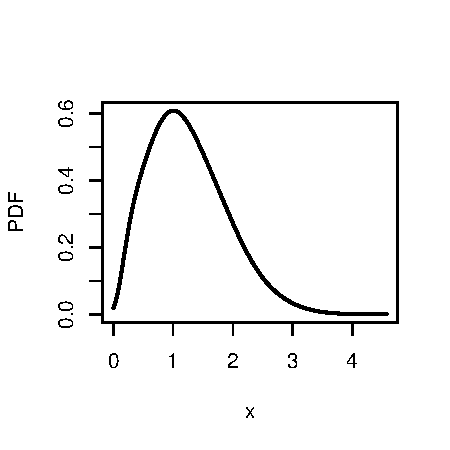
\includegraphics[width=2.0in, height=2.5in]{Figure3a.pdf} &
  \vspace{0pt} 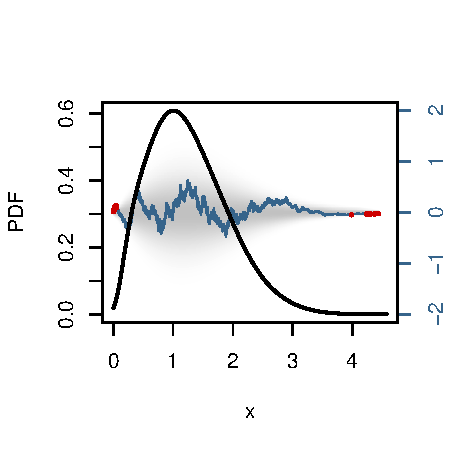
\includegraphics[width=2.0in, height=2.5in]{Figure3b.pdf} 
\end{tabular}
\caption{\label{fig:example1} (left) Density estimates for the Maxwell distribution with 100,000 samples using default parameters. (right) In addition to the density estimate, the scaled quantile residual mapped to the original variable x is shown along with a shaded region indicating 99\% target. The scaled quantile residuals outside of the 99\% target interval are highlighted in red.}
\end{figure}

Figure ~\ref{fig:example2} contains additional examples for visual assessment of estimates.  Each of these plots is based on the sawtooth distribution, defined by ten identical isosceles triangles at equal intervals. The sawtooth distribution is designed to be challenging to estimate due to these extremely sharp peaks. The exact distribution is plotted in gray in the top left panel of Figure~\ref{fig:example2}, with the \code{estimatePDF} estimate for 100,000 samples shown in black.  The estimate captures the high peaks well but falls short of reaching the lowest points of each triangle. The top right plot demonstrates how the \code{showOutlierPercent} parameter can identify specific areas of lower confidence in the estimate when the exact distribution is not known.  In this example, the estimate is plotted in gray with green highlighting the sample points outside of an 80\% target level.  Although the estimate closely approximates the distribution, the low peaks are identified as less accurate.

\begin{figure}[tbp]
\centering
\begin{tabular}{p{0.4\textwidth}p{0.4\textwidth}}
  \vspace{0pt} 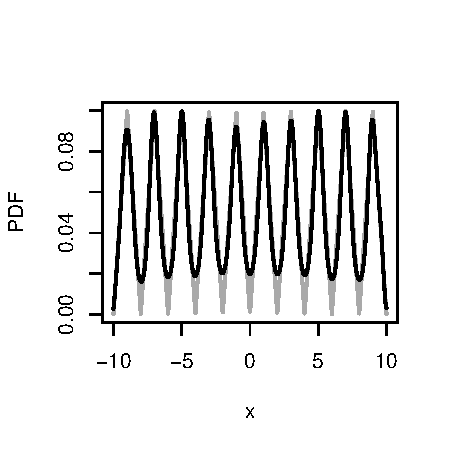
\includegraphics[width=2.2in, height=2.5in]{Figure4a.pdf} &
  \vspace{0pt} 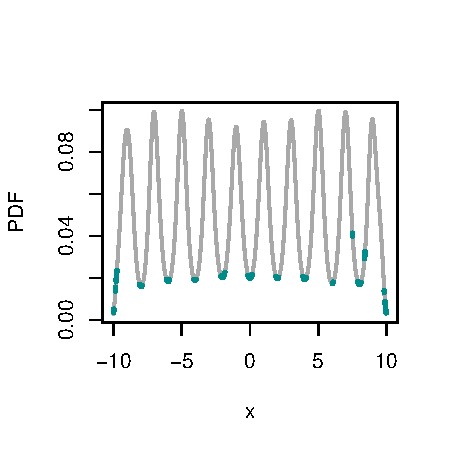
\includegraphics[width=2.2in, height=2.5in]{Figure4b.pdf} \\
  \vspace{0pt} 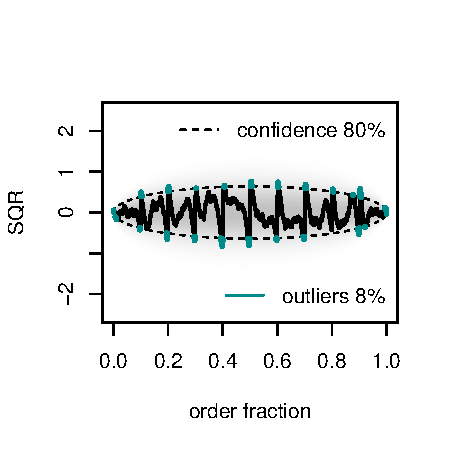
\includegraphics[width=2.2in, height=2.5in]{Figure4c.pdf} &
  \vspace{0pt} 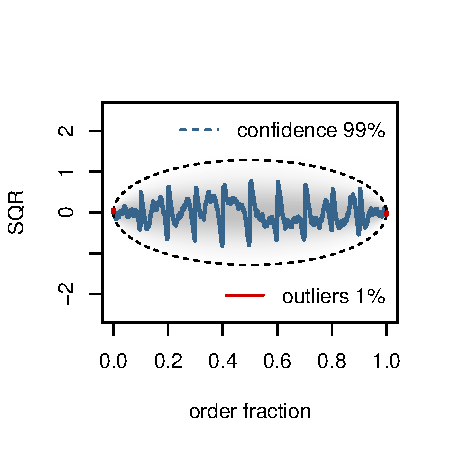
\includegraphics[width=2.2in, height=2.5in]{Figure4d.pdf} 
\end{tabular}
\caption{\label{fig:example2} Density estimates for the sawtooth distribution with 100,000 samples.  The top left plot shows the exact known distribution in gray and the estimate in black.  The top right plot shows the estimate in gray, with green highlights indicating areas outside of the 80\% target threshold. The bottom row demonstrates scaled quantile residual plots for the same estimate, for 80\% and 99\% target levels.}
\end{figure}

The bottom row of figure~\ref{fig:example2} shows an alternative diagnostic visualization of the same estimate.  These plots do not include the density estimate, but show only the SQR plot. Note that when the SQR is plotted alone, each sample point is spaced equally according to sort ordered position.  Additionally, dotted lines represent the confidence interval, if \code{showOutlierPercent} is specified, and the calculated percentage of points lying outside this threshold are printed on the bottom right.  These examples show targeted  thresholds of 80\% and 99\% with outliers representing 8\%  and 1\% of the points, respectively.  If the sum of the threshold and outlier percentages fall far below or above 100\%, this indicates a poor estimate. The figures in this section collectively demonstrate a wide range of visual assessment and color choices available with this customized \code{plot} function.



\subsection{Advanced diagnostics} \label{diagnostics}

The results returned from \code{estimatePDF} provide additional information for further analysis when needed. For example, the first plot in Figure~\ref{fig:normalcubed1} is the SQR result for 10,000 data samples generated from a normal-cubed distribution. In this case, the \code{failedSolution} return value is TRUE, indicating that the estimate does not meet the required threshold for the scoring function. Rather than return a NULL solution in the event of an unacceptable score, the best scoring estimate is always returned. However, in addition to the poor average score, the SQR plot also shows large variations outside of a 99\% threshold.

The second plot in Figure~\ref{fig:normalcubed1} shows the SQR result for the same sample data estimated with the core R function \code{density}.  The \code{density} estimate is first converted to a \code{PDFe} object via the \code{convertToPDFe} function. The \code{failedSolution} return variable indicates this estimate also does not meet an acceptable fit, but the SQR plot further suggests an extreme underfit of the estimate near the midpoint of the sample. This is a common weakness of KDE estimates for data with sharp peaks and long tails. In fact, the normal-cubed distribution is undefined at zero and diverges as it approaches this singularity from both directions, presenting a challenge for any density estimator. In either method, however, the information available in \code{PDFe} alerts the user of problems that may require intervention. 

A manual inspection of the sample data, perhaps in the form of a quantile or histogram plot, confirms an approximately symmetric distribution of data with an extreme variation in density near the center. A reasonable course of action in this event is to attempt to fit the low-density tails separately from the high-density peak.  Figure~\ref{fig:normalcubed2} demonstrates this approach, modeling the distribution with three separate calls to \code{estimatePDF} (top) and \code{density} (bottom) for ranges delineated by -0.01 and 0.01 around the peak. The tails are bounded according to the range returned from the respective original estimates for each method. 

For \code{estimatePDF}, this produces individual estimates mostly within the 99\% target range shown in the three SQR plots in Figure~\ref{fig:normalcubed2}. This example suggests a general divide and conquer method for addressing extreme distributions that is part of an automated procedure (to be published elsewhere). For \code{density}, however, the estimates remain poor in comparison even when fitting the regions separately. This is due, in part, because KDE methods do not incorporate automatic outlier detection. Additionally, KDE tends to perform poorly at boundaries, causing them to be less amenable to piecing together estimates in this way.

\begin{figure}[!htb]
\centering
\begin{tabular}{p{0.4\textwidth} p{0.4\textwidth}}
  \vspace{0pt} 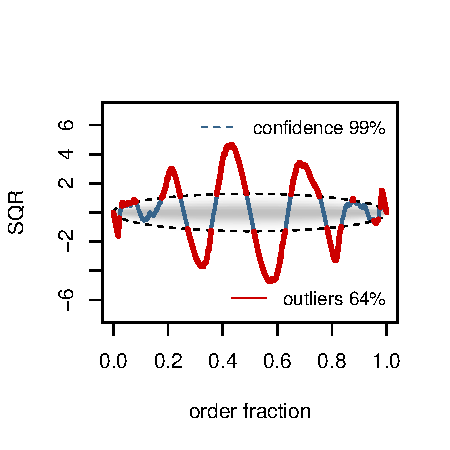
\includegraphics[width=2.2in, height=2.5in]{Figure5a.pdf} &
  \vspace{0pt} 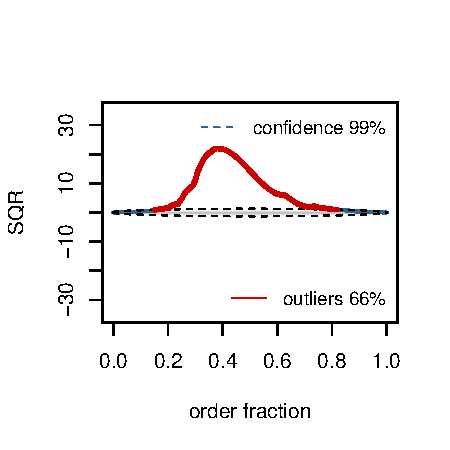
\includegraphics[width=2.2in, height=2.5in]{Figure5b.pdf} 
\end{tabular}
\caption{\label{fig:normalcubed1} Scaled quantile residual plots for estimates of the normal-cubed distribution with 10,000 samples using \code{estimatePDF} (left) and \code{density} (right).}
\end{figure}

\begin{figure}[tbp]
\centering
\begin{tabular}{p{0.3\textwidth} p{0.3\textwidth}p{0.3\textwidth}}
  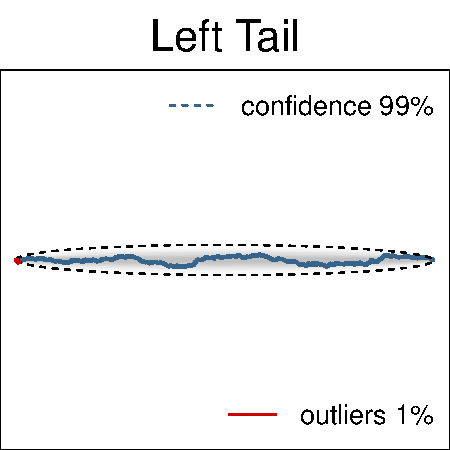
\includegraphics[width=1.55in, height=1.5in]{Figure6a.pdf} &
  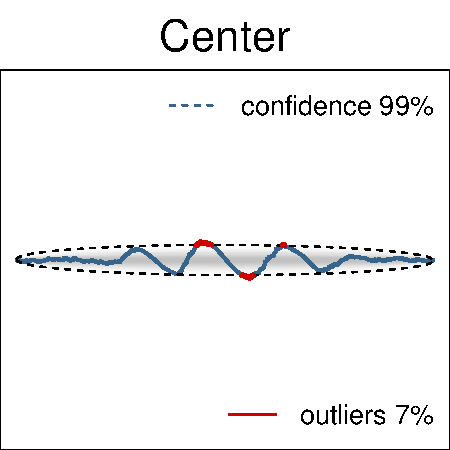
\includegraphics[width=1.55in, height=1.5in]{Figure6b.pdf} &
  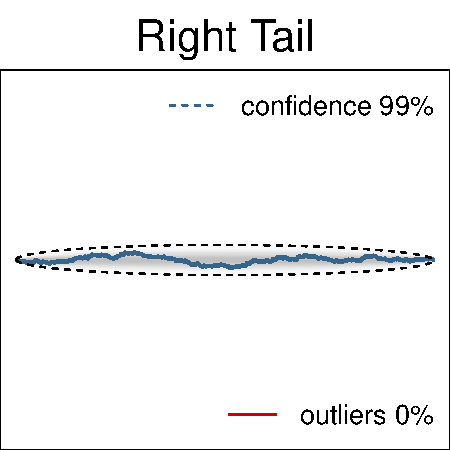
\includegraphics[width=1.55in, height=1.5in]{Figure6c.pdf} \\
  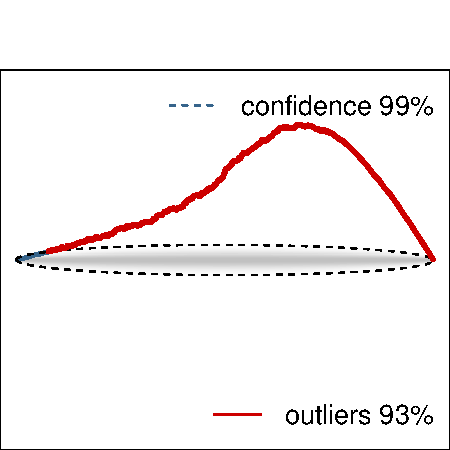
\includegraphics[width=1.55in, height=1.5in]{Figure6d.pdf} &
  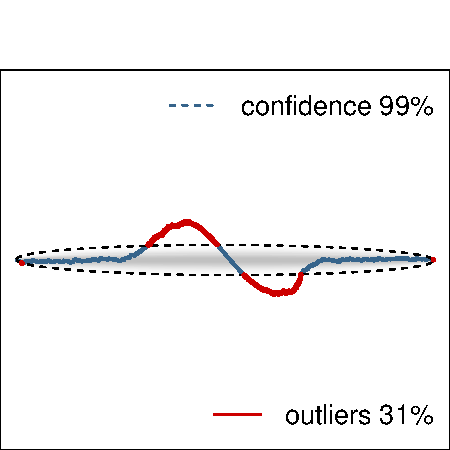
\includegraphics[width=1.55in, height=1.5in]{Figure6e.pdf} &
  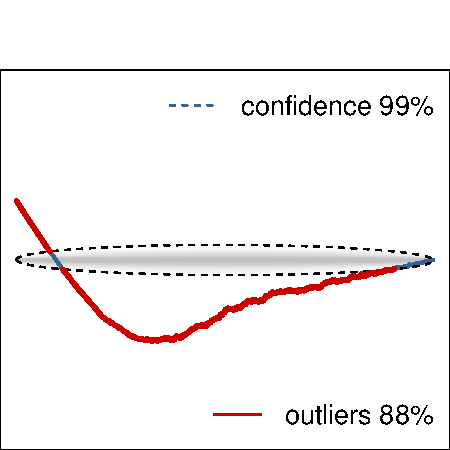
\includegraphics[width=1.55in, height=1.5in]{Figure6f.pdf} \\
\end{tabular}
\caption{\label{fig:normalcubed2} Scaled quantile residual plots for estimates of the normal-cubed distribution with 10,000 samples separated by left tail, middle, and right tail for \code{estimatePDF} (top row) and \code{density} (bottom row)}
\end{figure}

\section{Comparison to kernel-based estimators} \label{sec:comparison}

Conducting a fair comparison between nonparametric methods can be challenging due to the unrestrained nature of the input data. It is inevitable that different methods will do well estimating certain types of distributions while performing poorly on others.  The \CRANpkg{benchden} R package was implemented specifically to address this concern and facilitate an unbiased comparison between nonparametric methods \citep{benchden}. \pkg{Benchden} includes detailed information about a collection of 28 diverse known distributions, deliberately chosen to challenge estimation methods in a variety of ways, including long tails, discontinuities, and sharp or infinite peaks.  This data set is used to collect statistics on the accuracy, computational performance, and usability of \code{estimatorPDF} compared to several kernel-based methods.

Usability is admittedly somewhat subjective and difficult to measure.  An advanced user with in-depth knowledge of the data and experience with a particular method may choose to set parameters that differ from default values.  To control for
expert user biases, default settings are used across all methods.  Comparison functions were selected, in part, with the criteria that the only required user input is a data sample. However, all methods included in this comparison also allow optional parameters to specify finite boundary support for a distribution when provided by the \pkg{benchden} package.  Although many kernel-based functions were evaluated and tested, three representative methods were selected for the results in this section.  The first is \code{density}, the core R function. The other two are \code{npudens} and \code{bkde}, from the \CRANpkg{np} \citep{kdeR2} and \CRANpkg{KernSmooth} \citep{kernsmooth} packages, respectively.  These packages were also chosen to demonstrate specific advantages and features. 

Computational performance and accuracy comparisons are relatively straightforward to measure.  The R package \CRANpkg{philentropy} \citep{philentropy} implements 46 measurements designed specifically for comparing two distributions.  \pkg{Philentropy} was used together with \pkg{benchden} to generate random samples for each distribution and compare estimates for these samples against the known density.  For each of the four selected nonparametric methods, 100 random samples from each distribution available in \pkg{benchden} were estimated, timed, and averaged for sample sizes ranging from 10 to $10^6$ for all 46 accuracy measures in \pkg{philentropy}. All measurements were averaged first over 100 randomizations and then over all 28 distributions. 
Comparative results were qualitatively consistent between the 46 measures, particularly when averaged over a range of distributions, therefore, for simplicity, a single measure was selected for the plots in this section. A symmetric version of the chi-squared family was selected for the divergence, defined as 
\begin{equation} \label{eq:chi}
d=\sum_{i=1}^{n}\frac{\left(P_i - Q_i\right)^2}{P_i + Q_i}.
\end{equation}
Representative results for ten trials of each of the 28 distributions for select sample sizes are shown in the left plot of Figure~\ref{fig:compareDistributions1}. 

For functions \code {density}, \code{bkde}, and \code{estimatePDF}, the chi-squared error decreases with sample size while computational time, shown in the right plot of Figure~\ref{fig:compareDistributions1}, increases, as expected.  The relative comparison between these three methods shows that \code{estimatePDF}, on average, produces more accurate estimates at the expense of increased computational time. These trends generally agree with more comprehensive comparisons between \code{estimatePDF} and other nonparametric methods \citep{kdeR6}. \code{density} and \code{bkde} are very similar to one another, with \code{density} marginally slower and more accurate on average over \code{bkde}. The performance of \code{npudens} is less consistent.  The \pkg{np} package allows for an adaptive bandwidth selection that is the default method for \code{npudens}.  Although this functionality produces results with greater accuracy than \code{density} and \code{bkde}, it becomes computationally intractable as sample size increases.  The authors recommend against using the adaptive bandwidth option for sample sizes beyond 1000.  Simulations (not shown) were pushed to 50,000 samples at 100 trials, and 500,000 samples for a single trial, confirming the prediction of $O(n^2)$ time complexity for this method \citep{kdeR2}.

\begin{figure}[tbp]
\centering
\begin{tabular}{p{0.4\textwidth} p{0.4\textwidth}}
  \vspace{0pt} 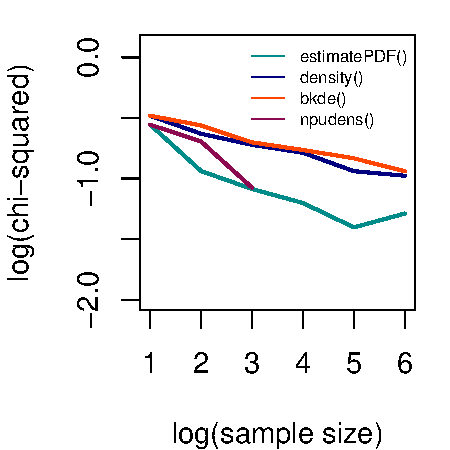
\includegraphics[width=2.2in, height=1.85in]{Figure7a.pdf} &
  \vspace{0pt} 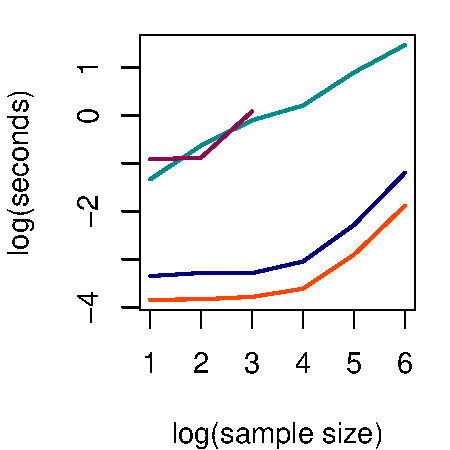
\includegraphics[width=2.2in, height=1.85in]{Figure7b.pdf} 
\end{tabular}
\caption{\label{fig:compareDistributions1} Comparison between four nonparametric estimators as a function of sample size according to accuracy (left) and performance (right). All quantities are averaged over 28 distributions for sample sizes in powers of 10.} 
\end{figure}

\begin{figure}[tbp]
\centering
\begin{tabular}{p{0.4\textwidth}p{0.4\textwidth}}
  \vspace{0pt} 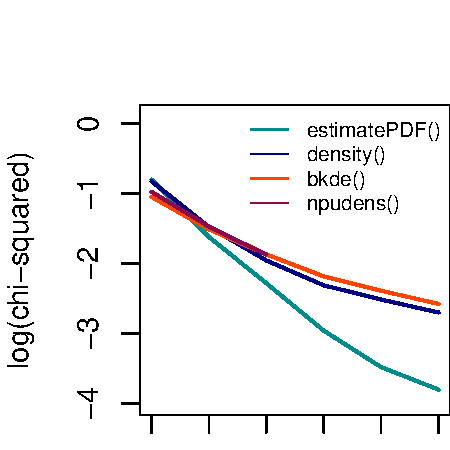
\includegraphics[width=2.1in, height=1.75in]{Figure8a.pdf} &
  \vspace{0pt} 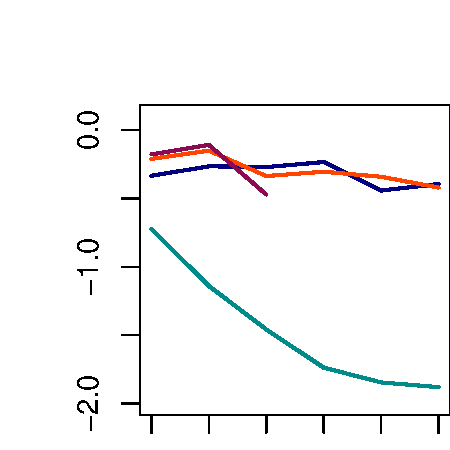
\includegraphics[width=2.1in, height=1.75in]{Figure8b.pdf} \\
  \vspace{0pt} 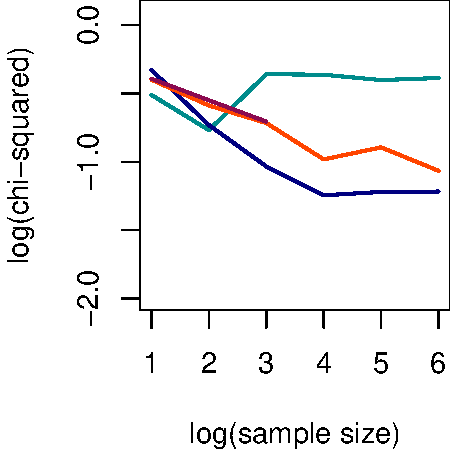
\includegraphics[width=2.1in, height=1.75in]{Figure8c.pdf} &
  \vspace{0pt} 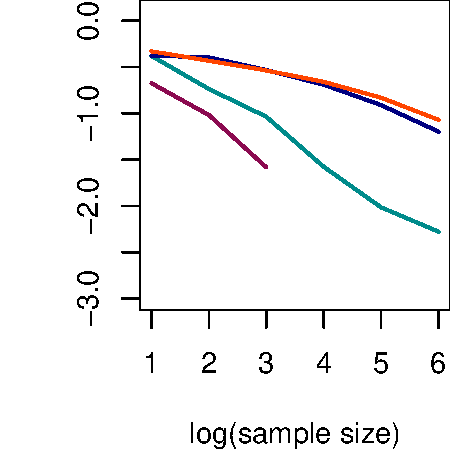
\includegraphics[width=2.1in, height=1.75in]{Figure8d.pdf} 
\end{tabular}
\caption{\label{fig:compareDistributions2} Accuracy comparison between four nonparametric estimators as a function of sample size averaged over subsets of distributions. Top left: distributions with high accuracy; top right: long tailed distributions; bottom left: Matterhorn and normal cubed distributions; bottom right: distributions with multiple peaks.}
\end{figure}

Although the plots in Figure~\ref{fig:compareDistributions1} provide an excellent snapshot of overall trends for comparison, a more detailed analysis per distribution is necessary for practical insight into the strengths and weaknesses of \code{estimatePDF} compared to the kernel-based estimates.  When viewing accuracy for each distribution separately, 12 of the 28 showed no significant differences between methods. When averaged over many trials, the magnitude of error empirically converges toward zero by approximately $n^{-0.56}$. The average chi-squared measures as a function of sample size for these 12 distributions are shown in the top left plot in Figure~\ref{fig:compareDistributions2}. Simple, well-behaved distributions are easy to estimate for all methods considered in this work.

The remaining plots in Figure~\ref{fig:compareDistributions2} illustrate more interesting cases where \code{estimatePDF} and kernel-based methods show their differences.  The top right plot, for example, is the accuracy averaged over four distributions (Cauchy, Pareto, symmetric Pareto, and inverse exponential) with extremely long tails.  Error remains high and somewhat erratic for all KDE methods, and visual inspection of the density plots reveal that they will often miss the location and density of the peak in favor of attempting to capture the low density in the tails.  The automatic boundary and outlier detection in the default behavior of \code{estimatePDF} correctly identifies the tails with near-zero density and removes them from consideration, thus fitting the peak extremely well with very little overall error in the estimate.

The bottom left plot in Figure~\ref{fig:compareDistributions2}, by contrast, shows the average accuracy of the two distributions (Matterhorn and normal-cubed) where \code{estimatePDF} performs poorly compared to the KDE methods. Although these distributions have quite different definitions, the common characteristics are that they are symmetrically distributed and are neither in $L_2$ nor $L_\infty$, with infinite peaks approaching zero from both directions.  This particular set of features is unique among the 28 distributions in \pkg{benchden}, and poses an exceptional challenge to \code{estimatePDF}. The Matterhorn distribution, by far the worst performer of the two, additionally suffers from known machine-precision errors in the random number generator in \pkg{benchden}, occasionally producing samples equal to zero where the distribution is undefined \citep{benchden}. Illustrative results from \code{estimatePDF} for the normal-cubed distribution were previously shown in Figure~\ref{fig:normalcubed1}, along with a demonstration of how a knowledgeable user can fit together segments of the data and combine the solutions to obtain a good estimate.

The bottom right plot in Figure~\ref{fig:compareDistributions2} highlights four distributions (sawtooth, smooth comb, Marronite, and claw) with multiple sharp peaks.  The adaptive bandwidth for \code{npudens} provides a clear advantage in accurately estimating these distributions over other KDE functions.  For small sample sizes, \code{npudens} also maintains an advantage over \code{estimatePDF}.  An example of this advantage is shown in the left panel of Figure~\ref{fig:sawtooth}, comparing \code{npudens} and \code{estimatePDF} for 1000 samples of the sawtooth distribution.  The right panel for Figure~\ref{fig:sawtooth} shows the estimates for this distribution at one million samples for \code{estimatePDF}, \code{density}, and \code{bkde}.  The two kernel-based estimates, processing in under 1 second, are quite poor.  The estimate for \code{estimatePDF}, taking about 1 minute, is notably improved and likely would be considered worth the additional computational investment to a user.  The \code{npudens} estimate, however, is projected to require 10-12 days to compute for 1 million samples, assuming the continuation of $O(n^2)$ time increase.  Any marginal increase in accuracy is unlikely to be worth the wait.

\begin{figure}[tbp]
\centering
\begin{tabular}{p{0.4\textwidth} p{0.4\textwidth}}
  \vspace{0pt} 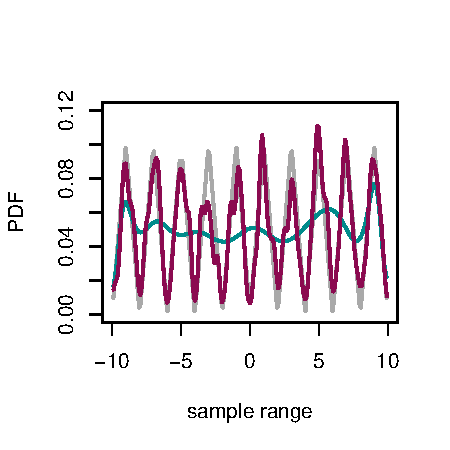
\includegraphics[width=2.0in, height=2.5in]{Figure9a.pdf} &
  \vspace{0pt} 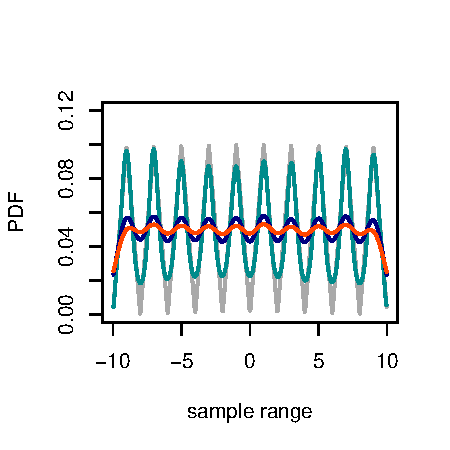
\includegraphics[width=2.0in, height=2.5in]{Figure9b.pdf} 
\end{tabular}
\caption{\label{fig:sawtooth} Left: Density estimates for the sawtooth distribution with 1000 samples for \code{estimatePDF} (green) and \code{npudens} (red).  Right: Density estimates for the sawtooth distribution with 1 million samples for \code{estimatePDF} (green), \code{density} (blue), and \code{bkde} (orange).}
\end{figure}

\section{The 1872 Hidalgo stamp issue of Mexico} \label{sec:stamps}

In 1988, Izenman and Sommer published a detailed statistical study and historical account describing a postage stamp collection issued in Mexico in 1872 \citep{stamp3}. This particular collection consists of only 485 stamps preserved from the millions originally issued that year, providing a very small and rare sampling of the data.  At this time in history, stamps were printed on a variety of paper types, with poor documentation and quality control on the thicknesses used for printing. Therefore, it is unknown how many paper types were used for this stamp issue in 1872, but those citing historical evidence and statistical analysis have estimated anywhere from 3 to 8 plausibly distinct thicknesses \citep{stamp1, stamp2, stamp3, stamp4}. 

A straightforward default estimate using the \code{density} function, shown in blue on the left plot of Figure~\ref{fig:stamp}, yields only two modes, with a bandwidth of 0.00391. Converting this estimate to a \code{PDFe} object calculates a threshold of only 0.27\% , indicating a very poor fit. By contrast, the \code{npudens} variable bandwidth estimate, shown in red, calculates a much smaller bandwidth at 0.00104 and includes at least 10 major and minor modes. Converting this estimate to a \code{PDFe} object yields a much more probable threshold of 56.4\%. More sophisticated parametric methods, such as mixed normal mode analysis, suggest that 7 modes is optimal \citep{stamp1, stamp3}.

The inherent difficulty in estimating real world data from such a small sample size is in distinguishing true characteristics of the data from random fluctuations of the sample. A unique advantage of \code{estimatePDF} is the ability to produce multiple viable solutions to fit the sample data. Since \code{estimatePDF} employs a random process for optimizing its parameters, starting with different seeds can result in a range of unique possible solutions consistent with the sampled data. When sample sizes become large, multiple solutions generally will converge to one single solution, but estimates for small sample sizes will generally have more variation. This application, where small features are of critical interest, provides an example of when the user may wish to deactivate the \code{smooth} functionality. Removing this penalty from the score will prioritize the most likely fit to the data with no regard to spurious noise in low-density areas.

This effect is demonstrated in the right plot of Figure~\ref{fig:stamp}. The results of 20 calls to \code{estimatePDF} are plotted in gray, and the average density over these 20 estimates is plotted in black. The average shows 7 smooth, distinct modes, corresponding to the 7 paper types proposed by Izenman and Sommer based on historical evidence. However, even with smoothing disabled, the two peaks in the right tail are very small and account for some amount of variation from one estimate to the next. There is some support, both historical and statistical, that these two modes are not justifiable, with some argument that there are only 5 modes \citep{stamp2, stamp4}. By contrast, the small mode between the largest two peaks on the left, seen in the \code{npudens} estimate and in some of the \code{estimatePDF} estimates, is generally agreed to be a random fluctuation of the sample set. \code{estimatePDF} demonstrates that these fluctuations are all possible fits to the data.


\begin{figure}[tbp]
\centering
\begin{tabular}{p{0.4\textwidth} p{0.4\textwidth}}
  \vspace{0pt} 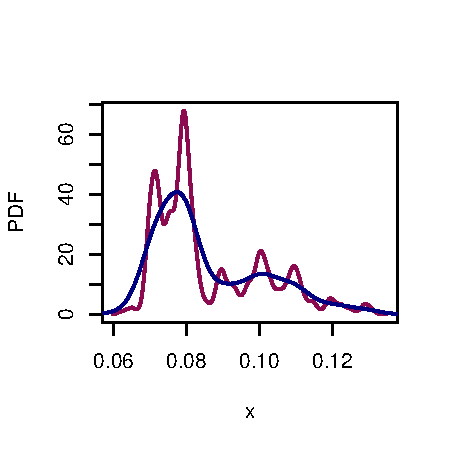
\includegraphics[width=2.0in, height=2.5in]{Figure10a.pdf} &
  \vspace{0pt} 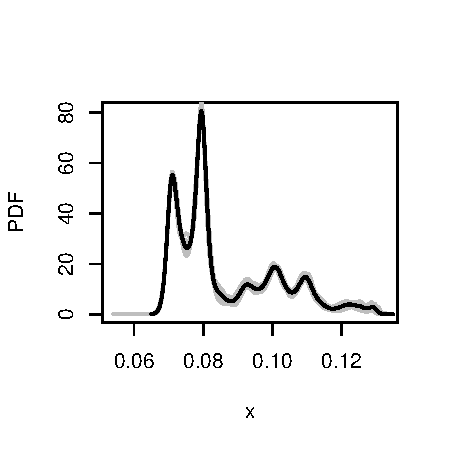
\includegraphics[width=2.0in, height=2.5in]{Figure10b.pdf} 
\end{tabular}
\caption{\label{fig:stamp} Estimates for the 1872 Hidalgo stamp issue of Mexico. (left) Default KDE estimate for \code{density} in blue, variable KDE estimate for \code {npudens} in red. (right) Multiple estimates for \code{estimatePDF} shown in gray, average in black.}
\end{figure}


\section{Summary} \label{sec:summary}

\pkg{PDFEstimator} is a probability density estimation package that introduces an R implementation of a novel nonparametric method, \code{estimatePDF}, based on maximum entropy. Any computational method must strike a reasonable balance between usability, computational time, and practical functionality. For comparison, \code{estimatePDF} was tested across a large range of random samples for 28 known distributions and compared to other popular R packages that implement nonparametric estimation through kernel density methods. Although specific results are problem-dependent, \code{estimatePDF} generally computes estimates much more quickly than those with competitive accuracy. Included in \pkg{PDFEstimator} is a collection of scoring assessments and plotting functions for displaying results and identifying problem areas in the estimate. These advanced plotting and analysis functions are independent of distribution type and estimation method and can be applied towards any density estimator in R. 

\bibliography{farmer_jacobs}

\address{Jenny Farmer\\
  Department of Bioinformatics\\
  University of North Carolina at Charlotte\\
  Charlotte, NC \\
  United States of America\\
  ORCiD 0000-0002-7953-1044\\
  \email{jfarmer@carolina.rr.com}}

\address{Donald Jacobs\\
  Department of Physics and Optical Science\\
  University of North Carolina at Charlotte\\
  Charlotte, NC \\
  United States of America\\
  ORCiD 0000-0001-7711-1639\\
  \email{djacobs1@uncc.edu}}


